\documentclass{standalone}

\usepackage[OT1]{fontenc}
\renewcommand*\familydefault{\sfdefault}
\usepackage{helvet,sfmath}
\usepackage{siunitx}

\usepackage{tikz}
\usetikzlibrary{arrows,calc,patterns}
\usepackage{tikz,tkz-euclide}
\usepackage{circuitikz}

%% Color %%
\definecolor{BlueDefault}{rgb}{0.2,0.2,0.7}
\definecolor{Fr4}{RGB}{228, 188, 65}
\definecolor{Copper}{RGB}{184, 115, 51}

\begin{document}

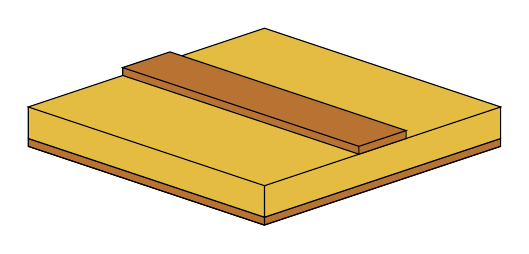
\begin{tikzpicture}[scale=1]
    % Ground
    \draw[fill = Copper]
    (0,0) to (0,0.1) to (3,1.1) to (3,1.0) to (0,0)
    (0,0) to (0,0.1) to (-3,1.1) to (-3,1.0) to (0,0)
    % (0,0.1) to (3,1.1) to (0,2.1) to (-3,1.1) to (0,0.1)
    ;
    \draw
    (0,0) to (3,1)
    (0,0) to (-3,1)
    ;
    % Substrate 1
    \draw[fill = Fr4]
    (0,0.1) to (0,0.5) to (3,1.5) to (3,1.1) to (0,0.1)
    (0,0.1) to (0,0.5) to (-3,1.5) to (-3,1.1) to (0,0.1)
    (0,0.5) to (3,1.5) to (0,2.5) to (-3,1.5) to (0,0.5)
    ;
    % Cut-wire
    % \draw[dashed]
    % (0,0.5) to (0,0.6) 
    % (0,0.5) to (0,0.6) 
    % (0,2.6) to (0,2.5)
    % (0,0.6) to (3,1.6) to (0,2.6) to (-3,1.6) to (0,0.6)
    % ;
    \draw[fill = Copper]
    % (0,1.4) to (0.6,1.6) to (0,1.8) to (-0.6,1.6) to (0,1.4)
    % (-0.6,2.0) to (-1.2,1.8) to (0.6,1.2) to (1.2,1.4) to (-0.6,2.0)
    (1.2,1.0) to (1.8,1.2) to (-1.2,2.2) to (-1.8,2.0) to (1.2,1.0)
    (1.2,1.0) to (1.8,1.2) to (1.8,1.1) to (1.2,0.9) to (1.2,1.0)
    (1.2,0.9) to (1.2,1.0) to (-1.8,2.0) to (-1.8,1.9) to (1.2,0.9)
    % (-1.2,1.8) to (0.6,1.2) to (0.6,1.1) to (-1.2,1.7) to (-1.2,1.8)
    % (0.6,1.2) to (0.6,1.1) to (1.2,1.3) to (1.2,1.4) to (0.6,1.2)
    ;
\end{tikzpicture}

\end{document}

